%---------------------------------------------------------------------------------------------------
% Realisierung
%---------------------------------------------------------------------------------------------------
\newpage
\chapter{Implementation}

In this chapter, the implementation phase is described in detail. After the fundamental design of the effect unit, all components are implemented separately in the first place. The following schematics and layouts are saved additionally on the attached CD\,(see \ref{DVD}).
During the realisation of the components, pre-testing approaches are reasonable to set adjustments for a good system performance.  

\section{Hardware Realisation}

\subsection{Preamp Module}

Figure \ref{fig:Preamp_schematic} shows the implemented circuit of the preamp module.
The following descriptions and calculations are partially adopted from the available Analysis\,\cite{ElectroSmash:2017}.

\begin{figure}[H]
\fbox{
	\centering 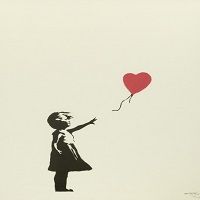
\includegraphics[width=1\textwidth]{banksy.jpg}
	}
	\caption[Preamp_schematic]{Schematic of preamp module}
	\label{fig:Preamp_schematic}
	
\end{figure}


\subsubsection{Power Supply and Interfaces}

Via a direct connection to the power switching supply output, the operating voltage of 12\,VDC is established. The TL071ACP is supplied by the 12\,VDC, whereas a voltage divider creates the needed 6\,VDC
bias voltage to ensure amplification of negative an positive signal amplitudes.

The preamp provides two 6.3\,mm mono audio jacks for the external interconnection of the effect unit, designed as unbalanced connections. A guitar output is supposed to be connected with the \textit{INSTRUMENT\_IN} - a guitar amplifier via \textit{INSTRUMENT\_OUT}.\\
For the unbalanced connection with the Audio-HAT two 3.5\,mm stereo audio jacks are implemented.
Due to the connection of the TIP-Pin only the left channel is used (mono).
The \textit{LINE\_OUT} is connected with the audio input of the HAT, \textit{LINE\_IN} receives the HAT's 
output signal.\\
\\




\subsubsection{Voltage Gain}
The original Micro-Amp is equipped with a gain regulator for an amplification between 0\,dB and 26,2\,dB. For the preamp module a fixed amplification is used, suitable for different passive guitars.
The goal is to raise the instrument level of the guitar to consumer audio line level.  
By a calculation done on a theoretical basis, the voltage gain can be assessed\,(\ref{eq:TheorectialGain}) assuming the RMS nominal levels\,(see section \ref{cap:TheoryLineLevel}).
\\
As a result of a practical pre-testing phase, the implemented voltage gain is set to 10,92\,dB (\ref{eq:ActualGain}). This avoids hearable clipping caused by unexpected voltage peaks of different types of guitar pickups and/or heavy strumming styles.

\begin{equation}
\mathrm{Gain}_{\mathrm{theoretical}}/\mathrm{dB} = 20 \cdot \mathrm{log} \bigg( \frac{0,316\,\mathrm{V}_{\mathrm{RMS}}}{0,072\,\mathrm{V}_{\mathrm{RMS}}} \bigg) \mathrm{dB}  = 12,85\,\mathrm{dB}
\label{eq:TheorectialGain}
\end{equation}

\begin{equation}
\mathrm{Gain}_{\mathrm{implemented}}/\mathrm{dB} = 20 \cdot \mathrm{log} \Bigg( \bigg( 1+ \frac{R_4}{R_5}\bigg) 
\cdot \bigg( \frac{R_7}{R_6+R_7}\bigg) \Bigg) \mathrm{dB}\ = 10,92\,\mathrm{dB}
\label{eq:ActualGain}
\end{equation}

The processed signal provided by the audio output from the HAT needs to be attenuated by the same factor.
A simple voltage divider formed by \textit{R8} and \textit{R9} is used\,(see \ref{eq:Loss}).
The implemented attenuation differs from an expected loss of -10,92\,dB, due to side effects of the Audio-HAT occurred in a practical test\,(see section \ref{cap:TestDistortion}). 

\begin{equation}
\mathrm{Loss}_/\mathrm{dB} = 20 \cdot \mathrm{log}  \bigg(  \frac{R_9}{R_8 + R_9} \bigg)  \mathrm{dB} = -11.04\,\mathrm{dB}
\label{eq:Loss}
\end{equation}

\subsubsection{Voltage Bridging}

In addition to the signal amplification, the required voltage bridging is guaranteed. For the interconnection with the guitar via \textit{INSTRUMENT\_IN} a suitable high input impedance is achieved
(\ref{eq:ZIn}). Provided by the 10$^{12}\,\Omega$ high JFET Input Stage resistance of the TL071ACP \cite{Tl071:2017}.\\

At the \textit{LINE\_OUT} a lower impedance is implemented to ensure maximum voltage transfer towards the HAT's audio input (\ref{eq:Zout}), based on the TL071ACPs internal output resistance of 192\,$\Omega$ according to the specification.\\ Both adjustments fulfil the required ratio between source and load impedance Z\,$_{\mathrm{load}} \geq$ 5 $\cdot$ Z\,$_{\mathrm{source}}$ (see section \ref{cap:TheoryVoltageBriding}).\\
\\
Guitar amplifiers commonly own a very high input impedance about 1\,M$\Omega$\footnote{URL: https://www.soundonsound.com/sound-advice/q-what-are-correct-input-impedances-guitars-and-mics/ [cited 06 September 2018]}. As a consequence the voltage bridging for the attenuation path between \textit{LINE\_IN} and \textit{INSTRUMENT\_OUT} is not further analysed. 


\begin{equation}
Z_{\mathrm{INSTRUMENT\_IN}} = \big( R_1 || R_2\big) \Big| \Big| \big( R_3 || Z_{\mathrm{ in,TL071ACP}}\big) = 5\,\mathrm{M}\Omega
\label{eq:ZIn}
\end{equation}

\begin{equation}
Z_{\mathrm{LINE\_OUT}} =  R_7 \Big| \Big| \big( R_6 || Z_{\mathrm{out,TL071ACP}}\big) = 657,64\,\Omega
\label{eq:Zout}
\end{equation}

\subsubsection{Frequency Response}

The preamp module is also equipped with four passive filters adopted from the MXR Micro-Amp to preserve its typical transparent and clean sound. These filters are not designed to cut-off relevant bass and treble frequency ranges of the characteristic guitar sound, but to eliminate low-frequency hum and harsh harmonics.
Four RC networks are used, designed as high pass or low pass. The objectives of these filters are not further described in the context of this thesis.

\begin{equation}
f_{\mathrm{cutoff},1} = \frac{1}{2\pi \Big( R_2 || (R_3 + Z_{\mathrm{in,TL071ACP}})\Big)} = 0,159\,\mathrm{Hz}
\label{eq:fc1}
\end{equation}

\begin{equation}
f_{\mathrm{cutoff},2} = \frac{1}{2\pi C_2 R_4} = 60,4\,\mathrm{kHz}
\label{eq:fc2}
\end{equation}

\begin{equation}
f_{\mathrm{cutoff},3} = \frac{1}{2\pi C_3 R_5} = 1,532\,\mathrm{Hz}
\label{eq:fc2}
\end{equation}

\begin{equation}
f_{\mathrm{cutoff},4} = \frac{1}{2\pi C_4 R_7} = 0,159\,\mathrm{Hz}
\label{eq:fc2}
\end{equation}


\subsubsection{PCB Design}

The layout of the preamp module is created with the Freeware version of \textit{EAGLE (Easily Applicable Graphical Layout Editor)} by \textit{Autodesk} \footnote{URL: https://www.autodesk.com/products/eagle/overview [cited 06 September 2018]}.
The resulting printed circuit board\,(PCB) layout is depicted in figure \ref{fig:Preamp_PCB}.
For the mechanical mounting of the preamp module four drill holes with the nominal diameter of 3\,mm are foreseen. In addition to that, the 6.3\,mm Audio jacks protrude over the edge for the direct mechanical coupling with the front panel of the case.\\
The assembled board is shown in figure \ref{fig:Preamp_Photo}.



\begin{figure}[H]
	\centering 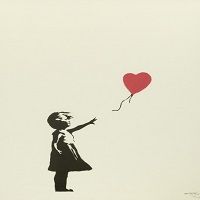
\includegraphics[width=0.75\textwidth]{banksy.jpg}
	\caption[Preamp_PCB]{PCB layout of preamp module}
	\label{fig:Preamp_PCB}
\end{figure}


\begin{figure}[H]
	\centering 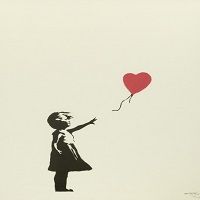
\includegraphics[width=0.75\textwidth]{banksy.jpg}
	\caption[Preamp_Photo]{Photo of preamp module}
	\label{fig:Preamp_Photo}
\end{figure}
% Used Eagle / maybe mention used own Parts
% show BRD and PHOTO
\newpage
\subsection{User Interface Module}\label{cap:hardwareUI}

For the connection of the chosen interface components\,(see section \ref{cap:designUI}) the 40 pin-header of the Raspberry Pi is used. As mentioned before 23 of 40 Pins are allocated by the Audio-HAT, thus 17 pins are available.\\
Acting as an intermediate element a module is implemented to unify common voltage potentials and provide enough space for needed additional resistors.
The Pi and the user interface periphery is connected via jumper cables with the module.
Figure \ref{fig:UI_schematic} shows the implemented board with the pin headers \textit{X1} to \textit{X6} for the periphery and \textit{X7} for the direct forwarding towards the Raspberry Pi.

\begin{figure}[H]
\centering 
	\fbox{
	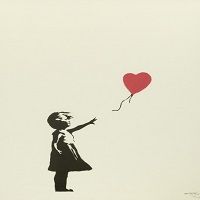
\includegraphics[width=0.7\textwidth]{banksy.jpg}
	}
	\caption[UI_schematic]{Schematic of user interface module}
	\label{fig:UI_schematic}
	
\end{figure}

\subsubsection{Rotary Encoders and Buttons}

The incremental rotary encoders KY-040 are equipped with five contacts. Besides the \textit{+} and \textit{GND} for the voltage supply, the two encoder signals \textit{CLK} and \textit{DT} are used to interpret the rotation direction.
The usage of the \textit{SW} contact, which is delivering a high signal when the encoder is pressed, is left out.\\
\\
For the interconnection of the rotary encoders and the buttons, suitable pull-up and/or pull-down resistors are
necessary. The appropriate debouncing is done on the software side.
The onboard PCB of the rotary encoders already provides two 10\,k$\Omega$ pull-up resistors for the encoder contacts \textit{CLK} and \textit{DT}.
Hence, \textit{X1} to \textit{X3} can be directly connected with the desired GPIO pin of \textit{X7}.
For the buttons on \textit{X4} and \textit{X5} two 10\,k$\Omega$ pull-down resistors are additionally implemented.

\subsubsection{Display}

The LCD 202A-Module is directly connected to the pin header \textit{X6}. The display generally is operating in 4\,bit or 8\,bit mode. In the context of this effect unit, a high update rate for the display is not required, so the benefit of a faster 8\,bit transfer can be neglected.
Therefore, and due to the limited GPIO pins of the Raspberry Pi, the display is connected in 4\,bit mode (see table \ref{tab:DisplayPins}).\\
For the adjustment of the LED backlight brightness, the resistor $R1$ is applied.
As a result of an experimental test with a potentiometer, a value of 470\,$\Omega$ delivers an appropriate brightness. For the LCD contrast adjustment $R2$ = 4,7\,k$\Omega$ turned out to be a suitable choice.


\begin{table}[H]
\begin{center}
\begin{tabular}{|c|c|c|p{6cm}|}
\hline 
\textbf{Pin} & \textbf{Symbol} & \textbf{Level} & \textbf{Description} \\ 
\hline 
\hline
1 & LED- & --- & Back light cathode \\ 
\hline 
2 & LED+ & --- & Back light anode \\ 
\hline 
3 & D7 & H/L & Data bit 7 \\ 
\hline 
4 & D6 & H/L & Data bit 6 \\ 
\hline 
5 & D5 & H/L & Data bit 5 \\ 
\hline 
6 & D4 & H/L & Data bit 4 \\ 
\hline 
7 & E & H/L & Enable signal \\ 
\hline 
8 & RW & H/L & H : Read mode, L : Write mode \\ 
\hline 
9 & RS & H/L & H : Data signal, L : Instruction signal \\ 
\hline 
10 & VEE &  --- & Input Voltage for LCD contrast \\ 
\hline 
11 & VDD & 5\,V & Supply voltage for logic \\ 
\hline 
12 & VSS & 0\,V & Ground \\ 
\hline 
\end{tabular} 
\end{center}
\caption{Interface pin connections of LCD 202A module \cite{LCD:2016}}
\label{tab:DisplayPins}
\end{table}

% Mention that this Module is necessary
% -> show Circuit and calculations (for resitors)
% LCD Resistors by Poti-Trying
\subsubsection{PCB Design}

The development of the PCB for the user interface module is comparable to the
construction of the preamp module.
Four drill holes with the nominal diameter of 3\,mm allow a tight mechanical coupling with the bottom plate of the case. Figure \ref{fig:UI_PCB} shows the PCB layout created with \textit{EAGLE}. The completely equipped board is depicted in Figure \ref{fig:UI_Photo}.
\begin{figure}[H]
	\centering 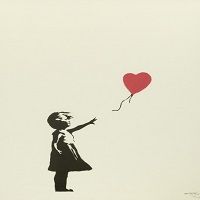
\includegraphics[width=0.8\textwidth]{banksy.jpg}
	\caption[UI_PCB]{PCB layout of user interface module.}
	\label{fig:UI_PCB}
\end{figure}

\begin{figure}[H]
	\centering 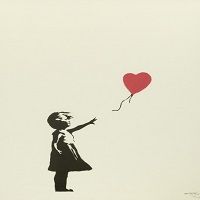
\includegraphics[width=0.8\textwidth]{banksy.jpg}
	\caption[UI_Photo]{Photo of user interface module}
	\label{fig:UI_Photo}
\end{figure}
% -> show BRD and PHOTO

\subsection{Construction of complete Unit}

All modules and components are placed inside the 19-inch case. The mounting is realised with fitting screws and nuts, except for the 230\,V power switch and the display which are fixed by a \textit{Snap-In} mechanism.\\
A total schematic of the effect unit is placed in the appendix\,(see figure  \ref{fig:UMLoverall}).



\subsubsection{Wiring of Power Supply}

For a secure and reliable electrical wiring of the 230\,V components, only \textit{H07V-K <VDE>} stranded wires with a diameter of 0,75\,mm$^2$ are used. In addition to that, suitable cable lugs and ferrules are applied as a standard in electrical enclosures.
For the power supply wiring of the extra low voltage components, these security regulations are not mandatory.

\subsubsection{Wiring of Signals}

The control signals are realized with the use of jumper cables, ideally for a fast and easy connection.
The resulting cable harness at pin headers $X1$ to $X6$ of the user interface module is bind together by cable ties. For the interconnection of the 40 pin header $X7$ with the Raspberry Pi, a ribbon cable is used as an ideal solution.

For the transmission of the audio signal from the preamp module to the Audio-HAT and back, unbalanced stereo audio cables are used. Suitable with the 3,5\,mm stereo audio jacks of the preamp module and the HAT its a forward-thinking choice for possible future extensions.
Figure \ref{fig:Unit_Inner} shows the total wiring of the effect unit.

\begin{figure}[H]
	\centering 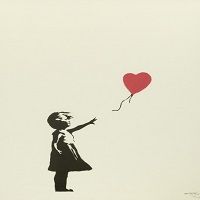
\includegraphics[width=0.9\textwidth]{banksy.jpg}
	\caption[Unit_Inner]{Top view of effect unit (without cover)}
	\label{fig:Unit_Inner}
\end{figure}

\subsubsection{Front Panel}
The placement of the components on the front panel is designed to gain maximum usability\,(figure \ref{fig:Unit_Front}).
The guitar signal input and output jacks are isolated on the left side. The display is centred on the front panel with a symmetrical formation of the rotary encoders below. As a consequence, the user is able to identify the corresponding rotary encoder for the variation of a parameter value.
The remaining components for the user controls are placed on the right side.

\begin{figure}[H]
	\centering 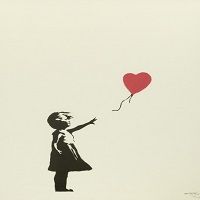
\includegraphics[width=0.9\textwidth]{banksy.jpg}
	\caption[Unit_Front]{Frontal view of effect unit (without cover)}
	\label{fig:Unit_Front}
\end{figure}





\section{Software Realisation}

In order to create a better overview, the implemented software can be separated into two elements: user interaction and audio signal processing. Both elements in combination are important to reach the goal of a fully working effect unit. The final program \textit{guitarEffects.c}\,(provided on the attached CD\,\ref{DVD}) is called via the \textit{rc.local} file of the Raspberry Pi, allowing the execution of the program while the Pi boots. Thus the effect unit is fully controlled via the user controls placed on the front panel.


\subsection{Audio Signal Processing}

The \textit{i2cDemo.c} program provided by Sebastian Albers\,\cite{Albers:2017} was originally developed for the demonstration of the signal processing capabilities of the HAT. The program forms a good basis for the implementation for the required guitar effects, by initializing ADC and DAC communication and setting up the audio performance parameters.\\
For the audio processing, the sampling rate $f_\mathrm{s}$ is set to 48\,kHz, fulfilling the demand of the Nyquist-Shannon sampling theorem (see equation \ref{eq:Nyquist}).
To ensure a high digital resolution, the bit depth is defined with 24\,bit.\\
The implementation of the guitar effects extends the \textit{i2cDemo.c} program by hearable and measurable sound changes. The manipulation of single samples is realised by taking advantage of the implemented FIFO\,(first in, first out) data buffer.
The communication between the ADC, DAC and the Raspberry Pi is based on the I$^2$S (Inter-IC Sound) serial bus.
For the left and right audio channel, a Pulse-code modulation (PCM) stream is provided.\\

% 48khz 24 bit 
% Explain sourcecode Principles of every Effekt
% (Refer to Theory Block)
% Describe every Parameter / Adjustment by hearing
% Calculation of Samples (24 Bit, LSB usw)
% hints for futre developers
% (Maybe source Code excerpts)
\subsubsection{Clean}
For the clean effect, the samples are not manipulated. The input samples are simply passed forward to the output.  


\subsubsection{Delay}

As depicted before in the block diagram (see \ref{fig:DelaySimple}) the delay a time-effect. An appropriate storage of input samples and the delayed addition with current input samples lead to the resulting output signal. In order to the requirements, a delay effect with three exemplary parameters is implemented.
Figure \ref{fig:ImplementedDelayBlock} shows the signal-flow graph to visualize the algorithm.
\\
\\
The \textit{level} parameter controls the general influence of the delay effect. As a factor placed at the end of the delay line it adjusts the total loudness of the delayed signal part.\\
For the variation of the fall time of the delayed samples, the \textit{decay} parameter is used.
Placed before the storage of input and delayed samples in the \textit{delayBuffer[]}, the \textit{decay} parameter can take the influence of the feedback path into account.
The actual delay time for every sample is controlled by parameter \textit{time}, defining the distance between the input and delayed sample in the time domain.

\begin{figure}[H]
	\centering 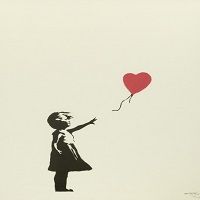
\includegraphics[width=0.9\textwidth]{banksy.jpg}
	\caption[ImplementedDelayBlock]{Signal-flow graph of implemented delay effect}
	\label{fig:ImplementedDelayBlock}
\end{figure}

Listing 5.1 shows an source code excerpt of the implemented function \textit{i2sDelayEffect()}.
The parameter values are controlled by the variables \textit{globalCounterParameter} set by the rotary encoders.
For a user-friendly control, the adjustable and displayed values are in the range of 1 to 10.
As a consequence, calculations are necessary for a suitable translation.
Parameter \textit{level} and \textit{decay} are implemented as factors, controlling the height of the amplitude in percentage between 0\,\% and 100\,\% (stepsize = 10\,\%).
The \textit{time} parameter is calculated with the sampling rate $f_\mathrm{s}$ and the fixed value 5000\,(see equation \ref{eq:CalcTime}), which leads to a total value range of 0\,ms to 1040\,ms (stepsize = 104\,ms).

\begin{equation}
\Delta t = \frac{\mathrm{globalCounterParameter} \cdot 5000}{f_\mathrm{s}} 
\label{eq:CalcTime}
\end{equation}



\fbox{
\lstinputlisting[caption={Excerpt of delay implementation},captionpos=b, language = c]{program/Delay.c}
}

\subsubsection{Distortion}

There is a wide range of possibilities to achieve a typical distorted guitar sound.
This distortion effect is implemented according to the description in table  \ref{tab:guitarEffects} and uses hard clipping. It is based on the analog method of placing two diodes antiparallel behind an amplifier connected to the ground. The amplitude of the guitar signal gets cut off by the time it reaches the threshold voltage of the diodes. As a consequence, the hard clipping leads to a very aggressive distorted guitar desired from many guitarists.\\
For this thesis, only one adjustable parameter for the threshold value is implemented for demonstration purposes.

The Audio-HAT is configurated with a bit depth of 24\,bit. According to the specification, the ADC \textit{PCM1864} \footnote{http://www.ti.com/lit/ds/symlink/pcm1864.pdf [cited 10 September 2018]} is equipped with a full-Scale input of 2,1\,V$_{\mathrm{RMS}}$.
So for the digital signal processing, the 0\,dBFS level is assigned to a maximum analog level of 2,969\,V$_{\mathrm{Peak}}$.
The DAC \textit{PCM514} provided the same value as a ground centred output. 
Based on that, the $U_{\mathrm{LSB}}$(voltage of the least significant bit) can be defined with equation \ref{eq:Ulsb}.


\begin{equation}
U_{\mathrm{LSB}} = \frac{U_{\mathrm{FS}}}{2^n}  = \frac{2 \cdot 2,969\,V}{2^{24}} = 3,539x10^{-7}\,\mathrm{V}
\label{eq:Ulsb}
\end{equation}

In a pre-testing phase with electric guitars for a suitable clipping-threshold, the hearable result was the most crucial factor. The distortion stages should vary in the range of 0 to 10 (from clean to slightly distorted and up to strongly distorted). A low threshold produces more hearable distortion by becoming a more square-wave-type signal.
Unfortunately, a linear relation between the thresholds led to a more unbalanced subdivision, in terms of subjective perception.\\
\\
Therefore the look-up table $\mathrm{factor\_table[n]}$ according to equation \ref{eq:LUTCalc} is implemented to get thresholds with a non-linear relation. As a result of a multiplication\,(\ref{eq:sampleValue}) of these factors with the fixed number 50000, sample values can be calculated. These values are representing the threshold voltage\,(see eq.\,\ref{eq:UThres}). 
Table \ref{tab:ThresValues} shows the translation of the $\mathrm{globalCounterParameter}$ controlled by the rotary encoder. Figure \ref{fig:ThresholdMATLAB} illustrates the performed hard clipping for every parameter in the time domain.


\begin{equation}
\mathrm{factor\_table[n]} = 30-9.25\sqrt{\mathrm{globalCounterParameter}}
\label{eq:LUTCalc}
\end{equation}

\begin{equation}
\mathrm{sampleValue} = \mathrm{factor\_table[n]} \cdot 50000
\label{eq:sampleValue}
\end{equation}

\begin{equation}
U_{\mathrm{Threshold}} = U_{\mathrm{LSB}}\cdot \mathrm{sampleValue}
\label{eq:UThres}
\end{equation}

\begin{table}[H]
\begin{center}
\begin{tabular}{|c|c|c|c|}
\hline 
 \textbf{globalCounterParameter} & \textbf{factor\_table[n]} & \textbf{sampleValue} & \textbf{$ \pm U_{\mathrm{Threshold}} /\mathrm{mV}$} \\ 
\hline 
\hline
1 & 20,75 & 1037500 & 367 \\ 
\hline 
2 & 16,62 & 846000 & 299 \\ 
\hline 
3 & 13,98 & 699000 & 247 \\ 
\hline 
4 & 11,5 & 575000 & 203 \\ 
\hline 
5 & 9,32 & 466000 & 165 \\ 
\hline 
6 & 7,34 & 367000 & 130 \\ 
\hline 
7 & 5,53 & 276500 & 98 \\ 
\hline 
8 & 3,84 & 192000 & 68 \\ 
\hline 
9 & 2,25 & 112500 & 40 \\ 
\hline 
10 & 0,75 & 37500 & 13 \\ 
\hline 
\end{tabular} 
\end{center}
\caption{Implemented distortion threshold values}
\label{tab:ThresValues}
\end{table}




\begin{figure}[H]
	\centering 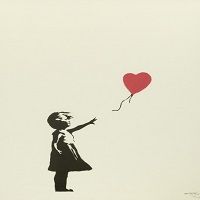
\includegraphics[width=0.8\textwidth]{banksy.jpg}
	\caption[Threshold]{Implemented hard clipping for globalCounterParameter 1 to 10}
	\label{fig:ThresholdMATLAB}
\end{figure}

After removing all values above the desired threshold, an adjustment is implemented to set the amplitudes to the same voltage level. The implement common level is lower than the original amplitude of the clean signal. This is necessary because the generated harmonics lead to a subjective louder sound.\\
In a pre-testing phase the adjustment-level is set to $\pm$ 160\,mV$_{\mathrm{Peak}}$. As a result, the distortion effect has a similar subjective loudness compared with the other effects. 

\subsection{User Interaction}

As described in \ref{cap:hardwareUI} all user interface components are connected via GPIO with the Raspberry Pi. Instead of an elaborate \textit{Direct Register Access}, the \textit{WiringPI} \footnote{https://github.com/WiringPi [cited 12 September 2018]} GPIO access library is used for an easy way of setting up, reading and writing the pins.\\
Moreover, \textit{WiringPI} includes an LCD library with helpful functions for the display communication. 

The pins allocated to the buttons and rotary encoders are set up as interrupts. Once requested, the audio processing is changed by an user interaction. As a consequence, the display is updated with the current status.\\
\\
In regard to the requirements, a user-friendly menu for the effect navigation is implemented\,(\ref{fig:Menu}).
After the effect unit is turned on with the \textit{Power ON/OFF} switch, the clean effect is executed. For this effect, no parameters are foreseen.
By pressing the \textit{Switch effect} button a new effect is called.
The display is showing the effect name and the three parameter values starting with the default value 5. These values are changeable by turning the corresponding rotary encoder.
For the delay effect the following parameters are assigned\,(from left to right): \textit{level - decay - time}.\\
Only the left parameter of the distortion effect is used for the threshold adjustment. The remaining can be interpreted as dummies. 
By pressing the \textit{Shut down} button at any time, the Pi can start shutting down. After about 5 seconds the voltage of the power switching supply needs to the interrupted manually by pressing the \textit{Power ON/OFF} switch.

\begin{figure}[H]
	\centering 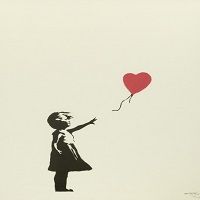
\includegraphics[width=1\textwidth]{banksy.jpg}
	\caption[Menu]{Diagram of user menu}
	\label{fig:Menu}
\end{figure}
% -> Activity Diagram of Menu with User Interaction 		%	(looking for solution)
% Explain User selections
% -> Show PHOTO of every Effect incl. Para Name.




